\documentclass[tikz,border=10pt]{standalone}
\usepackage{tikz}
\usetikzlibrary{shapes.geometric, arrows, positioning, fit, shadows}

\begin{document}

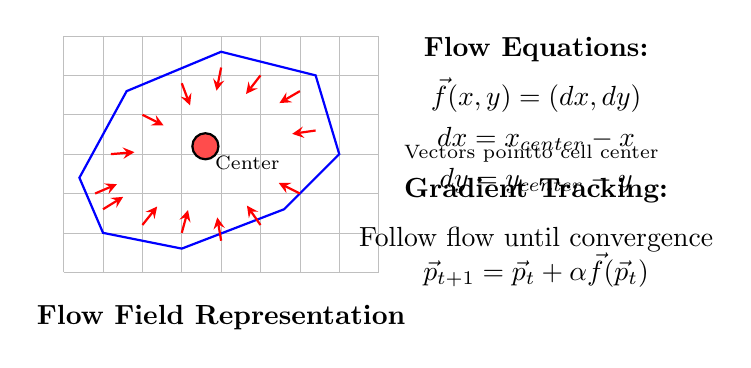
\begin{tikzpicture}[
    cell/.style={circle, draw, thick, fill=blue!30, minimum size=0.8cm},
    grid/.style={help lines, step=0.5cm, gray!50},
    arrow/.style={->, >=stealth, thick, red},
    center/.style={circle, draw, thick, fill=red!70, minimum size=0.3cm}
  ]

  % Grid
  \draw[grid] (0,0) grid (4,3);

  % Cell boundaries (rough outline)
  \draw[thick, blue] (0.5,0.5) -- (1.5,0.3) -- (2.8,0.8) -- (3.5,1.5) -- (3.2,2.5) -- (2.0,2.8) -- (0.8,2.3) -- (0.2,1.2) -- cycle;

  % Cell center
  \node[center] (center) at (1.8,1.6) {};

  % Flow vectors pointing to center
  \foreach \x/\y in {0.5/0.8, 1.0/0.6, 1.5/0.5, 2.0/0.4, 2.5/0.6, 3.0/1.0, 3.2/1.8, 3.0/2.3, 2.5/2.5, 2.0/2.6, 1.5/2.4, 1.0/2.0, 0.6/1.5, 0.4/1.0} {
      \pgfmathsetmacro{\dx}{1.8-\x}
      \pgfmathsetmacro{\dy}{1.6-\y}
      \pgfmathsetmacro{\len}{sqrt(\dx*\dx+\dy*\dy)}
      \pgfmathsetmacro{\ndx}{\dx/\len*0.3}
      \pgfmathsetmacro{\ndy}{\dy/\len*0.3}
      \draw[arrow] (\x,\y) -- +(\ndx,\ndy);
    }

  % Labels
  \node[below] at (2,-0.3) {\textbf{Flow Field Representation}};
  \node[right] at (4.2,1.5) {\scriptsize Vectors point\\to cell center};
  \node[below right] at (center) {\scriptsize Center};

  % Equations
  \node[align=center] at (6,2) {
    \textbf{Flow Equations:}\\[0.2cm]
    $\vec{f}(x,y) = (dx, dy)$\\[0.1cm]
    $dx = x_{center} - x$\\[0.1cm]
    $dy = y_{center} - y$
  };

  \node[align=center] at (6,0.5) {
    \textbf{Gradient Tracking:}\\[0.2cm]
    Follow flow until convergence\\
    $\vec{p}_{t+1} = \vec{p}_t + \alpha \vec{f}(\vec{p}_t)$
  };

\end{tikzpicture}

\end{document}
